\chapter{Sound-wave characterization}
\label{app:SoundWaveCharacterization}
\begin{itemize}
  \item Sound-wave dispersion relation
\end{itemize}


\section{Hardware}
\label{sec:SoundWaveCharacterization:Hardware}
\subsection{Speaker}
\label{sec:SoundWaveCharacterization:Hardware:speaker}
\subsection{Calibrated microphone}
\label{sec:SoundWaveCharacterization:Hardware:microphone}
\subsection{Test stand}
\label{sec:SoundWaveCharacterization:Hardware:test_stand}


\section{Sound-wave measurements}
\label{sec:SoundWaveCharacterization:Measurements}
To lowest order, the speaker is cylindrically symmetric.
Thus, the sound waves are expected to have
axial, radial, and frequency dependencies.
Sections~\ref{sec:SoundWaveCharacterization:Measurements:amlitude} through
\ref{sec:SoundWaveCharacterization:Measurements:phasing}
summarize these measurements and their implications
for the sound-wave model developed in
Section~\ref{sec:SoundWaveCharacterization:Model}.


\subsection{On-axis amplitude}
\label{sec:SoundWaveCharacterization:Measurements:amlitude}
After centering the microphone on the speaker's symmetry axis,
the on-axis amplitude can be easily characterized by
varying both the frequency $f$ of the sound waves and
the microphone height $z$ above the speaker face.
The frequencies $f$ and heights $z$
are motivated by the parameters of the heterodyne interferometer
described in Chapter~\ref{ch:Implementation}.
Specifically, the interferometer spatial bandwidth
$|k| \leq \SI{5}{\per\centi\meter}$
from (\ref{eq:Implementation:kfsv_interferometer_design}) motivates
sound-wave measurements at frequencies
$f \lesssim \SI{30}{\kilo\hertz}$
(i.e.\ $|k| \lesssim \SI{5}{\per\centi\meter}$).
Further, to produce a robust interference signal
during sound-wave calibrations,
the speaker is placed very close
to the edge of the collimated probe beam,
which has 1/e $E$ radius $w_0 = \SI{3.4}{\centi\meter}$;
thus, sound-wave measurements are made at heights
spanning the probe-beam profile
$z
=
\{\SI{2.5}{\centi\meter}, \SI{5.5}{\centi\meter}, \SI{8.5}{\centi\meter}\}$.
The on-axis amplitude of the sound waves as a function of
wavenumber $k$ and height $z$ above the speaker face is shown in
Fig.~\ref{fig:SoundWaveCharacterization:tymphany_on_axis_amplitude}.
As expected, the on-axis amplitude decreases with
increasing distance $z$ from the speaker face.
Further, the on-axis amplitude has a complicated wavenumber dependence, but
it is relatively flat for
$\SI{1}{\per\centi\meter} \lesssim k \lesssim \SI{3.5}{\per\centi\meter}$.

\begin{figure}
  \centering
  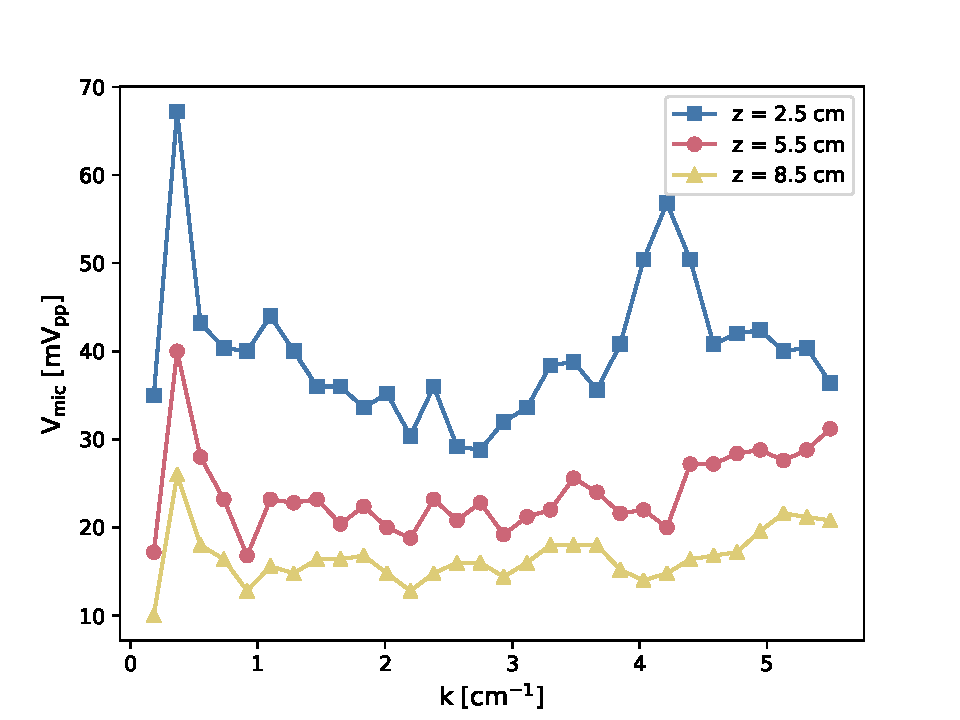
\includegraphics[width = \textwidth]{%
    Appendices/SoundWaveCharacterization/figs/tymphany_on_axis_amplitude.pdf}
  \caption[On-axis amplitude of sound waves]{%
    On-axis amplitude of sound waves as a function of
    wavenumber $k$ and height $z$ above the speaker face.
    Note that the amplitude is specified
    as a \emph{peak-to-peak} value.
  }
\label{fig:SoundWaveCharacterization:tymphany_on_axis_amplitude}
\end{figure}


\subsection{Wavefront phasing}
\label{sec:SoundWaveCharacterization:Measurements:phasing}
Characterizing the sound-wave phasing is somewhat more involved
than characterizing the on-axis amplitude,
as it requires measurements at several radial positions $\rho$
for each frequency $f$ and microphone height $z$.
For this reason, the wavefront-phasing measurements
are more coarsely sampled in frequency $f$
than the on-axis amplitude measurements in
Section~\ref{sec:SoundWaveCharacterization:Measurements:amlitude}.
For a given frequency $f$ and height $z$,
the sound-wave phasing is measured by
tracking a point of constant phase in the microphone waveform
as the radial position $\rho$ is varied;
such tracking can be easily accomplished
by triggering the oscilloscope
with a copy of the waveform that is driving the speaker.
To begin the radial scan,
the microphone height $z$ is selected, and
the microphone is displaced from the speaker's symmetry axis
by a few centimeters.
Then, in $\SI{1}{\centi\meter}$ increments,
the microphone is moved radially inwards towards the center;
upon passing through the center,
the radial scan is continued in $\SI{1}{\centi\meter}$ increments
until the sound-wave amplitude becomes negligible.
Note that beginning the radial scan
with a small displacement from the symmetry axis
allows empirical identification of the symmetry-axis location
(by e.g.\ fitting the measured amplitude and/or phasing
and identifying the extremum that occurs at the symmetry axis).

\begin{figure}
  \centering
  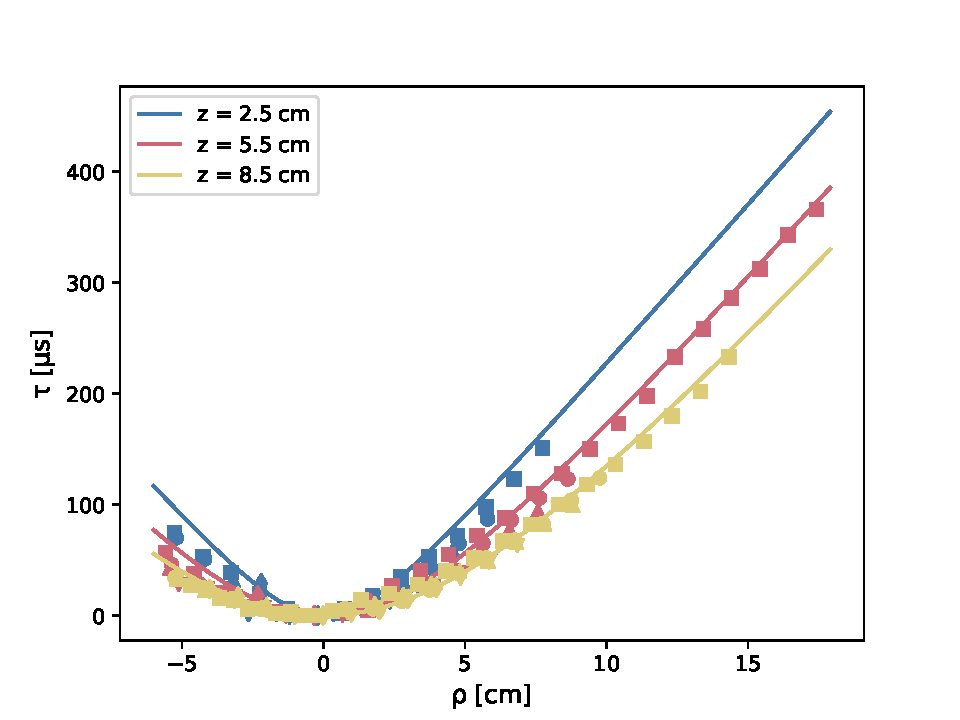
\includegraphics[width = \textwidth]{%
    Appendices/SoundWaveCharacterization/figs/tymphany_wavefront_phasing.pdf}
  \caption[Wavefront phasing of sound waves]{%
    Wavefront phasing of sound waves.
    The symbols show the measured time delay $\tau$
    between the wavefront at height $z$ and radial displacement $\rho$ and
    the corresponding on-axis wavefront (i.e.\ same $z$ but $\rho = 0$),
    with each symbol shape corresponding to particular frequency.
    The traces correspond to the time delay
    (\ref{eq:SoundWaveCharacterization:time_delay})
    predicted for spherical waves.
    The close proximity of the measured points to the spherical-wave traces
    indicates that, to lowest order, the waves are approximately spherical
    over the spatial domain and frequencies probed.
  }
\label{fig:SoundWaveCharacterization:tymphany_wavefront_phasing}
\end{figure}

At sufficiently large distances,
the speaker will behave like a point source,
producing sound waves with spherical wavefronts.
This point-source approximation is taken as a reasonable
starting point for the investigation of the wavefront phasing.
If a sound wave is measured on axis at height $z$ above the speaker,
the corresponding wavefront will subsequently arrive
at position $r = (z^2 + \rho^2)$
delayed by a time $\tau$
\begin{equation}
  \tau = \frac{r - z}{c_s},
  \label{eq:SoundWaveCharacterization:time_delay}
\end{equation}
\graffito{\textcolor{red}{value for $c_s$}}
where $c_s$ is the sound speed.
Fig.~\ref{fig:SoundWaveCharacterization:tymphany_wavefront_phasing}
compares the measured time delay to
the time delay predicted for spherical waves
(\ref{eq:SoundWaveCharacterization:time_delay})
as a function of height $z$, radial position $\rho$, and frequency $f$.
Clearly, to lowest order, the waves are approximately spherical
over the spatial domain and frequencies probed.


\subsection{Spatial envelope}
\label{sec:SoundWaveCharacterization:Measurements:envelope}
If the sound-wave amplitude is also measured
during the radial scans described in
Section~\ref{sec:SoundWaveCharacterization:Measurements:phasing},
the spatial envelope of the sound waves can also be quantified.
Fig.~\ref{fig:SoundWaveCharacterization:tymphany_spatial_envelope_z_5_5cm}
displays the spatial envelopes of sound waves of various frequencies $f$
at height $z = \SI{5.5}{\centi\meter}$ above the face of the speaker.
Clearly, the width of the spatial envelope decreases
with increasing frequency $f$.
Measurements at other heights $z$
exhibit qualitatively similar behavior.

\begin{figure}
  \centering
  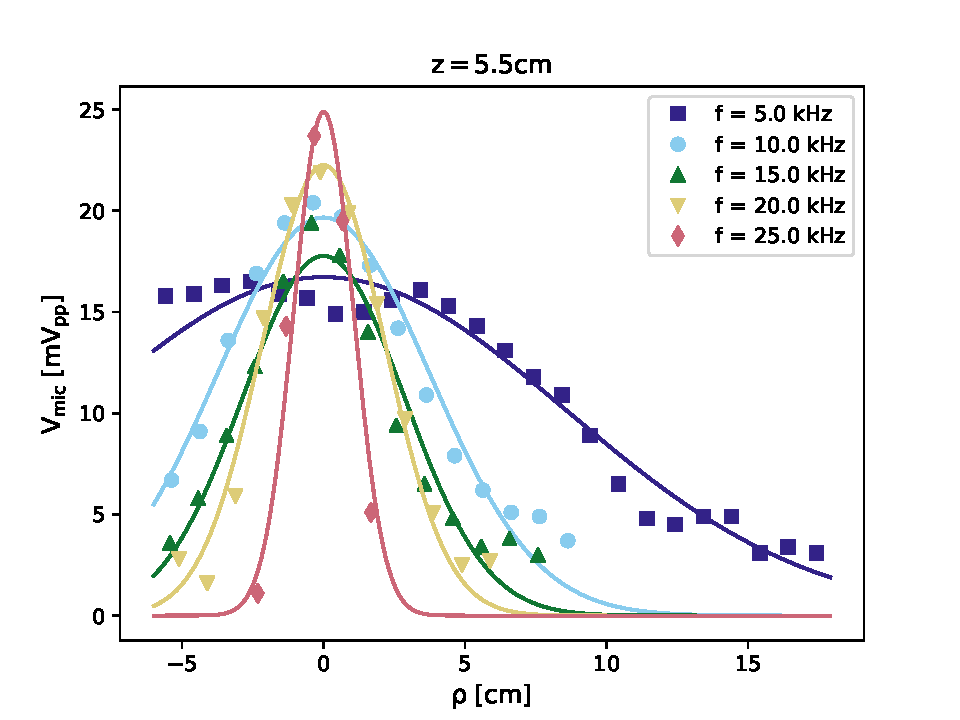
\includegraphics[width = \textwidth]{%
    Appendices/SoundWaveCharacterization/figs/tymphany_spatial_envelope_z_5_5cm.pdf}
  \caption[Representative spatial envelopes of sound waves]{%
    Sound-wave spatial envelopes for frequencies $f$
    at height $z = \SI{5.5}{\centi\meter}$ above the face of the speaker.
    Symbols indicate measurement points, while
    the traces correspond to Gaussian fits of the form
    (\ref{eq:SoundWaveCharacterization:Gaussian}).
    Measurements and fits at other heights $z$
    exhibit qualitatively similar trends.
  }
\label{fig:SoundWaveCharacterization:tymphany_spatial_envelope_z_5_5cm}
\end{figure}

The narrowing of the spatial envelope with increasing frequency
can be quantified by fitting the measurements
to an assumed functional form.
To lowest order, the spatial envelopes are well approximated by a Gaussian
\begin{equation}
  V_{\text{mic}}(\rho)
  =
  V_0(z, f)
  \exp\left[
    \frac{-\rho^2}{w(z, f)^2}
  \right],
  \label{eq:SoundWaveCharacterization:Gaussian}
\end{equation}
where $w(z, f)$ is the 1/e radius, which
is a function of the height $z$ and the sound-wave frequency $f$.
Gaussian fits to the envelope measurements are also shown in
Fig.~\ref{fig:SoundWaveCharacterization:tymphany_spatial_envelope_z_5_5cm}.
Deviations from a Gaussian are most apparent at low frequencies;
this may be attributable to baffle diffraction across the speaker face but
was not further investigated.
The approximation of a Gaussian envelope
will be sufficiently accurate for the present work.
Fig~\ref{fig:SoundWaveCharacterization:tymphany_gaussian_widths}
displays the fitted 1/e Gaussian radii $w$ as a function of
sound-wave wavenumber $k$ and
height $z$ above the face of the speaker.
As previously and anecdotally noted for $z = \SI{5.5}{\centi\meter}$,
the width of the spatial envelope $w$
decreases with increasing $k$ for each height $z$.
Further, $w$ increases with increasing $z$, which
results from free-space diffraction of the sound wave.

\begin{figure}
  \centering
  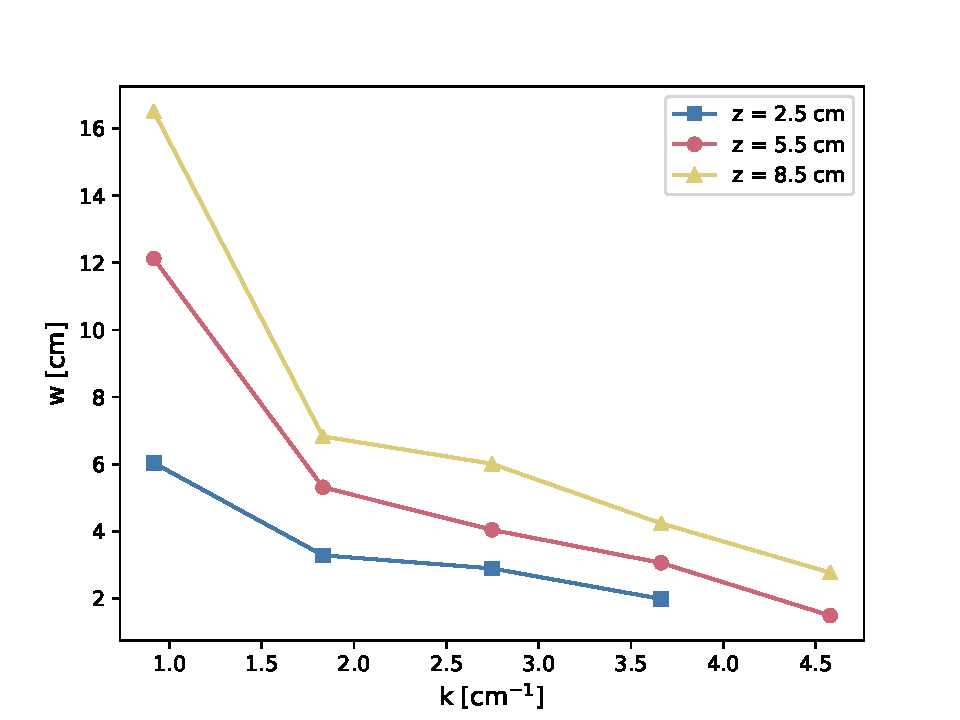
\includegraphics[width = \textwidth]{%
    Appendices/SoundWaveCharacterization/figs/tymphany_gaussian_widths.pdf}
  \caption[Gaussian widths of sound waves]{%
    Fitted 1/e Gaussian radii $w$ of sound waves
    as a function of sound-wave wavenumber $k$ and
    height $z$ above the face of the speaker.
  }
\label{fig:SoundWaveCharacterization:tymphany_gaussian_widths}
\end{figure}


\section{Sound-wave model}
\label{sec:SoundWaveCharacterization:Model}


\section{Perturbed index of refraction}
\label{sec:SoundWaveCharacterization:PerturbedIndexOfRefractiion}


\bibliographystyle{plainurl}
\bibliography{references}
